\documentclass[a4paper]{article}



\usepackage{Sweave}
\begin{document}
\Sconcordance{concordance:test.tex:test.rnw:%
1 4 1 1 0 4 1 1 2 4 0 1 2 1 1 1 2 1 0 1 1 3 0 1 2 3 1 1 -6 1 0 1 1 1 8 %
1 1 19 0 1 1 4 0 1 2 2 1}



First we define a figure hook:
\begin{Schunk}
\begin{Sinput}
> options(SweaveHooks = list(fig = function() par(mfrow=c(2,2))))
\end{Sinput}
\end{Schunk}

Then we setup variable definitions without actually evaluating them
\begin{Schunk}
\begin{Sinput}
> x <- 1:10
> y <- rnorm(x)
\end{Sinput}
\end{Schunk}


Then we put the pieces together:
\begin{center}
\begin{Schunk}
\begin{Sinput}
> x <- 1:10
> y <- rnorm(x)
> lm1 <- lm(y~x)
> summary(lm1)
\end{Sinput}
\begin{Soutput}
Call:
lm(formula = y ~ x)

Residuals:
    Min      1Q  Median      3Q     Max 
-1.0721 -0.6070 -0.2778  0.6116  1.3101 

Coefficients:
            Estimate Std. Error t value Pr(>|t|)
(Intercept) -0.45078    0.58744  -0.767    0.465
x            0.09297    0.09467   0.982    0.355

Residual standard error: 0.8599 on 8 degrees of freedom
Multiple R-squared: 0.1076,	Adjusted R-squared: -0.00398 
F-statistic: 0.9643 on 1 and 8 DF,  p-value: 0.3549 
\end{Soutput}
\begin{Sinput}
> plot(lm1)
\end{Sinput}
\end{Schunk}
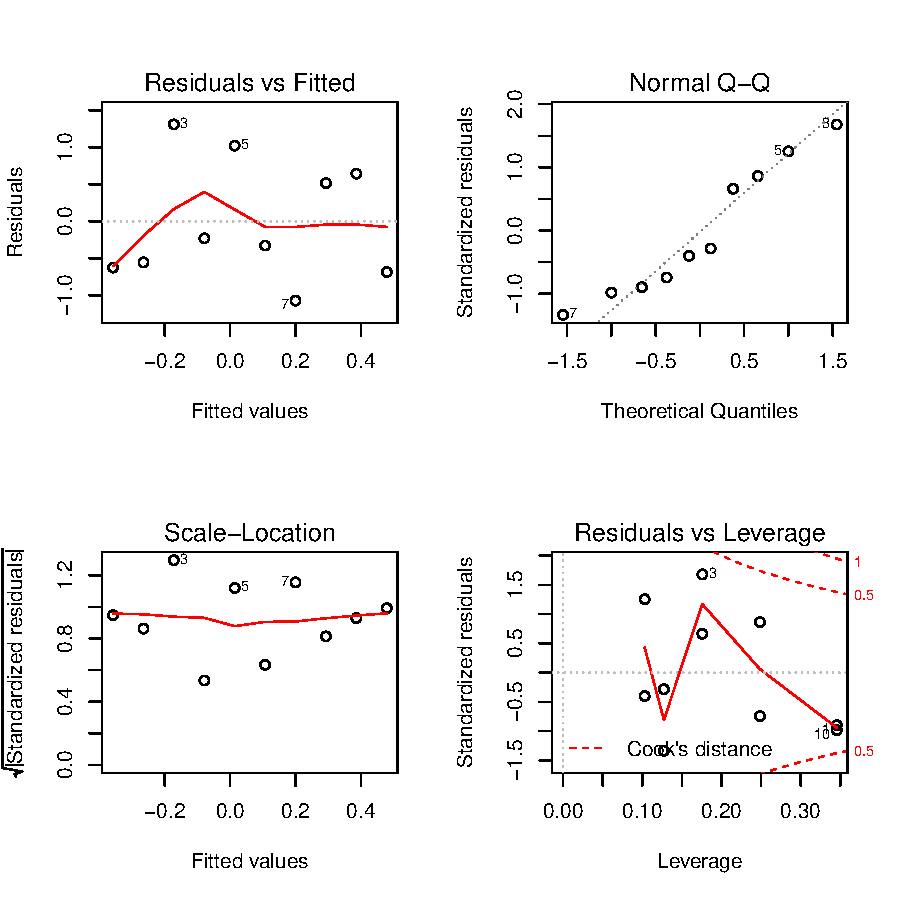
\includegraphics{test-003}
\end{center}

\end{document}
